\documentclass{article}
\usepackage[left=0.25in, right=0.25in, top=0.75in, bottom=0.75in]{geometry}
\usepackage{mathtools,amssymb}
\usepackage{enumerate}
\usepackage{algorithm2e}
\usepackage{graphicx}
\usepackage{subfigure}
\usepackage{fancyhdr}
\usepackage{cancel}
\usepackage{titling}
\usepackage{tcolorbox}
\usepackage{listings}
\usepackage{xcolor}
\usepackage{caption}
\usepackage{hyperref}
\usepackage{lmodern}
\usepackage{placeins}
\usepackage{multirow}
\usepackage{csvsimple}
\usepackage{tikz}

%%%%%%%%%%% Tikz settings optimized for causal graphs.
\usetikzlibrary{shapes,decorations,arrows,calc,arrows.meta,fit,positioning,backgrounds,petri}
\tikzset{
    -Latex,auto,node distance =1 cm and 1 cm,semithick ,
    state/.style ={ellipse, draw, minimum width = 0.7 cm},
    point/.style = {circle, draw, inner sep=0.04cm,fill,node contents={}},
    bidirected/.style={Latex-Latex,dashed},
    el/.style = {inner sep=2pt, align=left, sloped}
}
%%%%%%%%%%%
\usepackage{cleveref}

\pagestyle{fancy}

\hypersetup{%
  colorlinks=true,
  linkbordercolor=red,
  linkcolor=blue,
  pdfborderstyle={/S/U/W 1}% border style will be underline of width 1pt
}

%%%%%%% DEFINE CODE STYLE HERE
\definecolor{mygreen}{rgb}{0,0.6,0}
\definecolor{mygray}{rgb}{0.5,0.5,0.5}
\definecolor{mymauve}{rgb}{0.58,0,0.82}

\lstset { 
  backgroundcolor=\color{white},   % choose the background color; you must add \usepackage{color} or \usepackage{xcolor}; should come as last argument
  basicstyle=\footnotesize,        % the size of the fonts that are used for the code
  breakatwhitespace=false,         % sets if automatic breaks should only happen at whitespace
  breaklines=true,                 % sets automatic line breaking
  captionpos=b,                    % sets the caption-position to bottom
  commentstyle=\color{mygreen},    % comment style
  deletekeywords={...},            % if you want to delete keywords from the given language
  escapeinside={\%*}{*)},          % if you want to add LaTeX within your code
  extendedchars=true,              % lets you use non-ASCII characters; for 8-bits encodings only, does not work with UTF-8
  firstnumber=1,                % start line enumeration with line 1000
  frame=tbRl,	                   % adds a frame around the code
  keepspaces=true,                 % keeps spaces in text, useful for keeping indentation of code (possibly needs columns=flexible)
  keywordstyle=\color{blue},       % keyword style
  language=Java,                 % the language of the code
  morekeywords={*,...},            % if you want to add more keywords to the set
  numbers=left,                    % where to put the line-numbers; possible values are (none, left, right)
  numbersep=5pt,                   % how far the line-numbers are from the code
  numberstyle=\tiny\color{mygray}, % the style that is used for the line-numbers
  rulecolor=\color{black},         % if not set, the frame-color may be changed on line-breaks within not-black text (e.g. comments (green here))
  showspaces=false,                % show spaces everywhere adding particular underscores; it overrides 'showstringspaces'
  showstringspaces=false,          % underline spaces within strings only
  showtabs=false,                  % show tabs within strings adding particular underscores
  stepnumber=1,                    % the step between two line-numbers. If it's 1, each line will be numbered
  stringstyle=\color{mymauve},     % string literal style
  tabsize=4,	                   % sets default tabsize to 2 spaces
  title=\lstname                   % show the filename of files included with \lstinputlisting; also try caption instead of title
}

%%%%%%%%%%%%%%%%%%%%%%%%%%

\newcommand{\soln}{\\ \textbf{Solution}: }
\newcommand{\bkt}[1]{\left(#1\right)}

%%%%%%% DEFINE HEADER HERE
\lhead{CS6235: Analysis of Parallel Programs}
% \chead{Assignment: 1}
\rhead{Roll No: CS17B046}
%%%%%%%%%%%%%%%%%%%%%%%%%%

%%%%%%% DEFINE TITLE HERE
\title{Written Assignment 1}
\author{Vimarsh Sathia}
%%%%%%%%%%%%%%%%%%%%%%%%%%

\begin{document}
  \maketitle
	\thispagestyle{fancy}
	\section{Non-atomicity with and without data races}
    
    \subsection{Data Race Snippet}
      \Cref{code::11} has a data race in the access of variables \lstinline!reward! and \lstinline!num_workers! in their respective \lstinline!get! and \lstinline!set! methods. \\
      This is also observed in the output screenshot in \Cref{fig::11}.

      \lstinputlisting[caption={Code of datarace.java (\lstinline!cheatDay()! and \lstinline!addPushups()! are called in different threads)}, label={code::11}]{1_datarace/datarace.java}

      \begin{figure}[h]
        \centering
        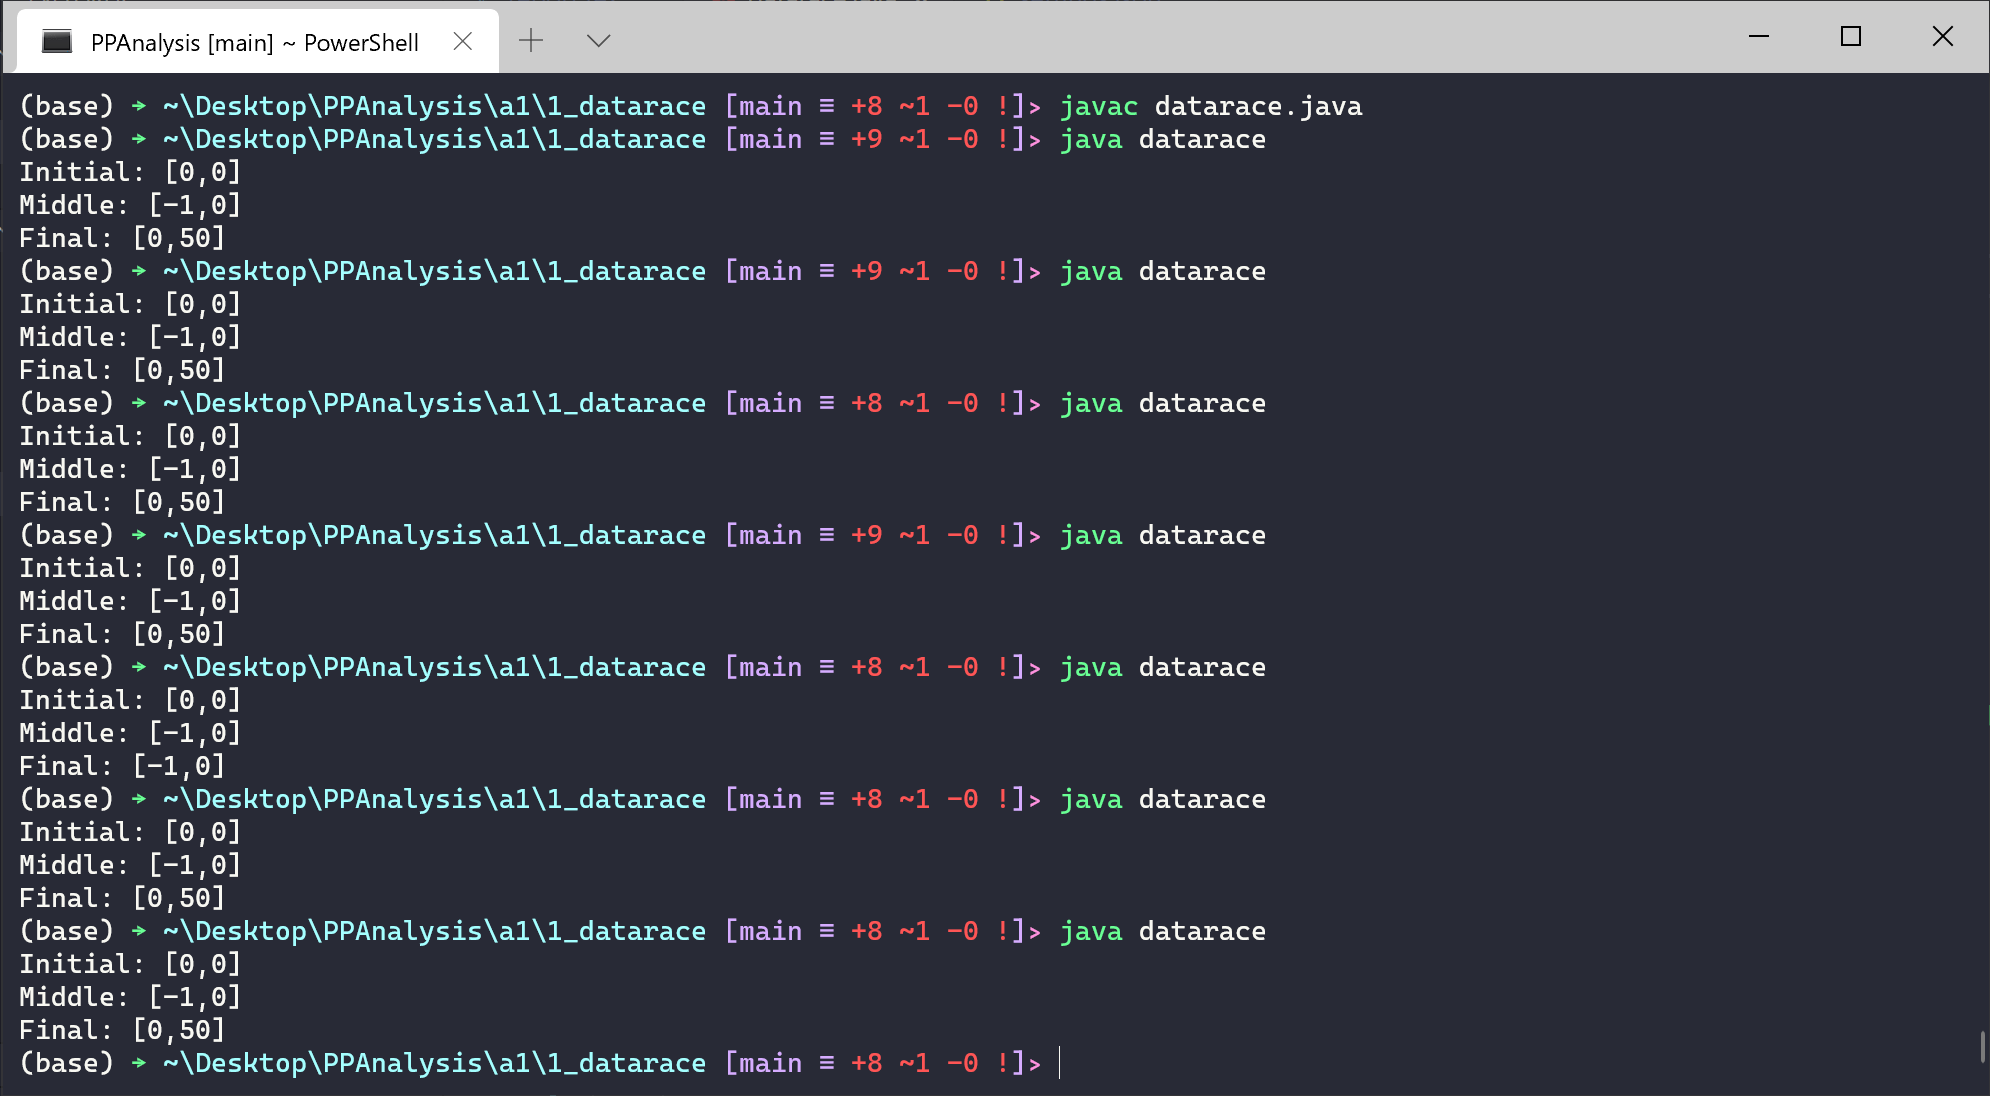
\includegraphics[scale=0.7]{1_datarace/datarace_output.png}
        \caption{Screenshot of output showing inconsistent results between runs.}
        \label{fig::11}
      \end{figure}
    
    \subsection{Data Race-free snippet}

      In \Cref{code::12}, the variables \lstinline!reward! and \lstinline!num_workers! are accessed exclusively in a synchronized method. Hence there are no data-races between threads \lstinline!t! and \lstinline!main!. \\
      However even in this case, atomicity of \lstinline!addPushups()! and \lstinline!cheatDay()! is not gauranteed, since reads and writes may be interleaved between both the running threads.\\
      This behaviour can be observed in \Cref{fig::12}.

      \lstinputlisting[caption={Code of dataracefree.java (\lstinline!cheatDay()! and \lstinline!addPushups()! are again called in different threads)}, label={code::12}]{1_datarace/dataracefree.java}
      
      \begin{figure}[h]
        \centering
        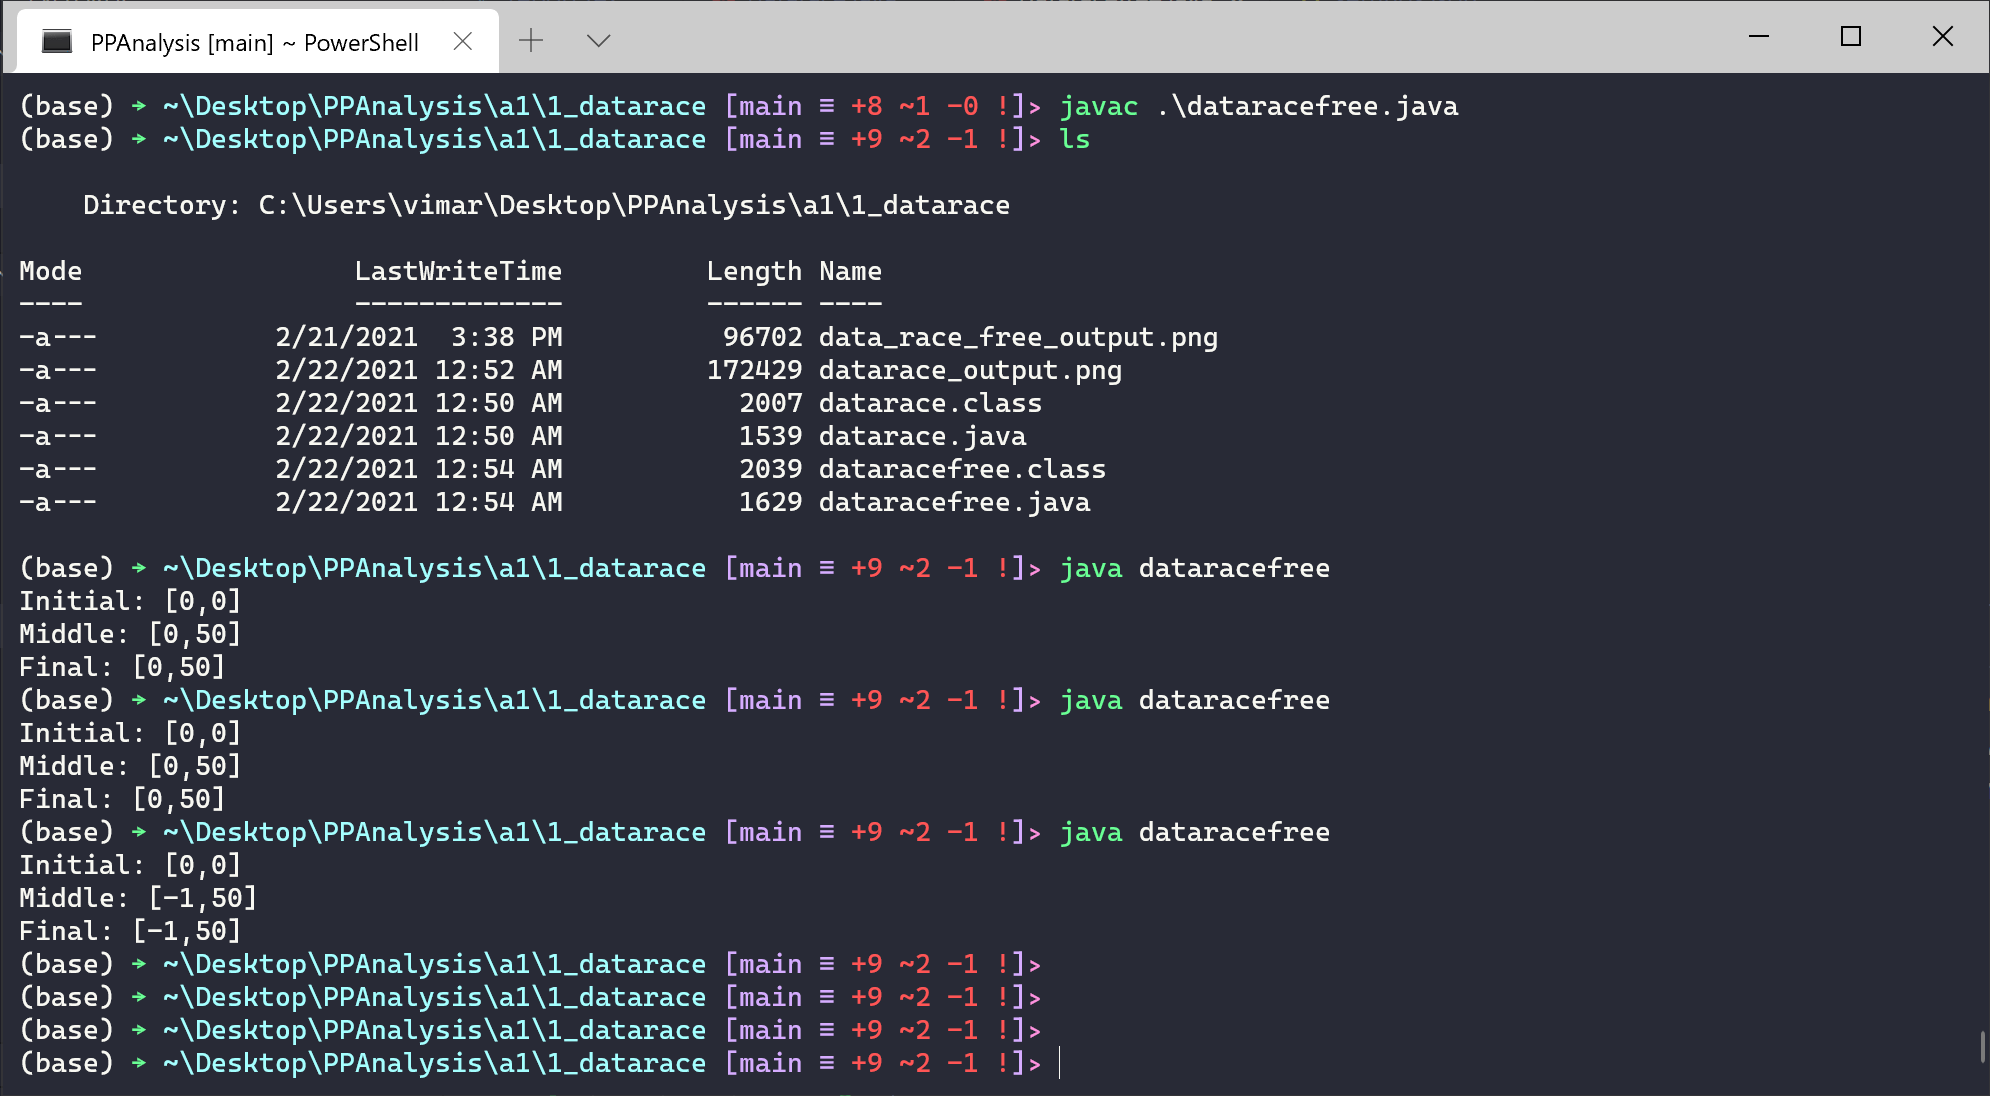
\includegraphics[scale=0.7]{1_datarace/dataracefree_output.png}
        \caption{Screenshot of inconsistent results, despite the variables being accessed by a single thread at a time (race-free)}
        \label{fig::12}
      \end{figure}
      
  % \clearpage
  \section{Verification of Amdahl's law}
    Amdahl's law states that the total speedup of a program is ultimately decided by the non-parallelizable portion of the porgram. \\
    To verify this, the snippet in \Cref{code::21} performs a modified parallel version of the \href{https://developer.nvidia.com/blog/six-ways-saxpy/}{\textbf{saxpy}} routine and calculates execution time and speedups by varying the number of threads.\\
    The execution time for every thread configuration was taken as the mean of $10$ runs, with all statistics compiled into \textbf{benchmarks.csv}. A plot of the execution speedup w.r.t the mean single threaded computation time is also provided in \Cref{fig::21}.

    \lstinputlisting[caption={Code for parallelization of the \textbf{saxpy} operation with \lstinline!num_workers! threads}, label={code::21}]{2_amdahl/Saxpy.java}

    \begin{figure}[h]
      \centering
      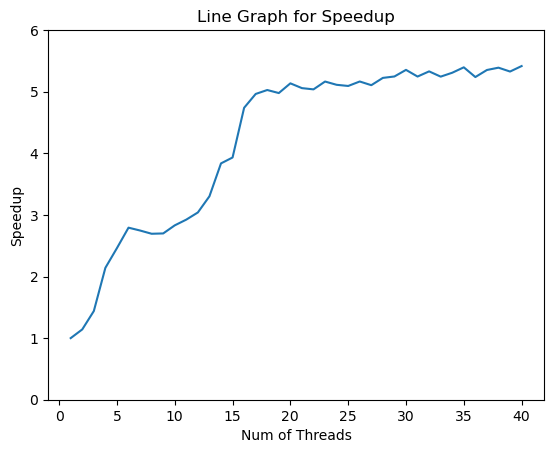
\includegraphics[scale=0.5]{2_amdahl/speedup_graph.png}
      \caption{Graph of mean speedup as a function of the number of threads. We see that for more number of threads, the speedup plateaus out. The exact timing values are recorded in \href{run:./2_amdahl/benchmarks.csv}{benchmarks.csv}}
      \label{fig::21}
    \end{figure}
  % \clearpage
  \section{Java threads share the heap}
    We show that java threads share the heap using the snippet in \cref{code::31} and it's corresponding output in \cref{code::32}.\\
    Since the list is in heap memory, and all thread names are reflected in it, we can conclude that java threads share the heap.

    \lstinputlisting[caption={Code for showing java threads share the heap in \lstinline!heapshare.java! }, label={code::31}]{3_heapshare/heapshare.java}

    \lstinputlisting[caption={Output of the code in \cref{code::31}},label={code::32}]{3_heapshare/output.txt}

  % \clearpage
  \section{Happens Before Relation between statements}
    In this section, the statement at line $i$ is represented as $S_i$. If there is a happens before relation from the action on line $i$ to line $j$, it is represented as $S_i$ HB $S_j$ 
    \subsection{For \textit{datarace.java}}
      For \textit{datarace.java} whose snippet is provided in \Cref{code::11}, we have the following happens-before relations.
      \begin{itemize}
        \item \textbf{Main thread:}
          \[
            S47 \rightarrow S48 \rightarrow S49 \rightarrow S36 \rightarrow \mathbf{S38} \rightarrow S39 \rightarrow S40 \rightarrow S23 \rightarrow S9 \rightarrow S24 \rightarrow S12 \rightarrow S25 \rightarrow S10 \rightarrow S26 \rightarrow S13 \rightarrow S41 \rightarrow \mathbf{S42} \rightarrow S50 
          \]
        \item \textbf{Spawned thread:}
          \[
            \mathbf{S38} \rightarrow S31 \rightarrow S32 \rightarrow S16 \rightarrow S9 \rightarrow S17 \rightarrow S12 \rightarrow S18 \rightarrow S10 \rightarrow S19 \rightarrow S13 \rightarrow \mathbf{S42}
            \]
      \end{itemize}
      There are no happens-before relations between the threads, and thus there is a data race in the access of \lstinline!this.reward! and \lstinline!this.num_workers!.

    \subsection{For \textit{dataracefree.java}}
      For \textit{datarace.java} whose snippet is provided in \Cref{code::12}, we have the following happens before relations \textbf{in addition to the ones defined previously}. Note that $S9, S10, S12$ and $S13$ are accessed through a synchronized method lock on the main object in this snippet.
      \begin{figure}[h]
      \centering
      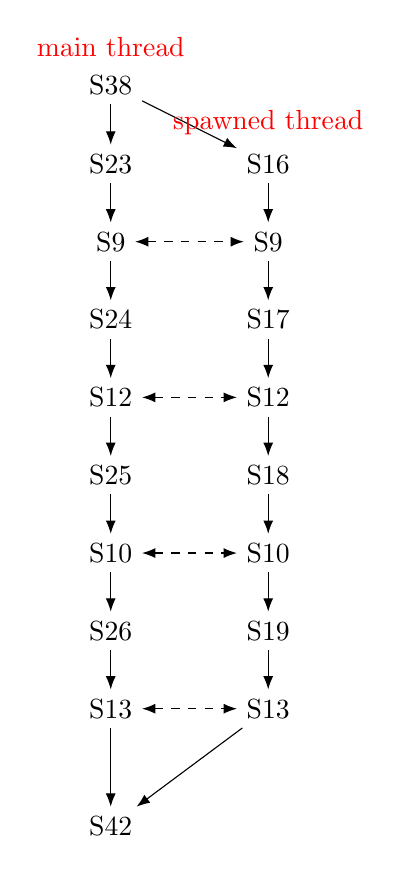
\begin{tikzpicture}
        \node (1) at (-1,0) {S38};
        \node (a) at (-1,-1) {S23};
        \node (b)[below=0.5cm of a] {S9}; 
        \node (c)[below=0.5cm of b] {S24};
        \node (d)[below=0.5cm of c] {S12};
        \node (e)[below=0.5cm of d] {S25};
        \node (f)[below=0.5cm of e] {S10}; 
        \node (g)[below=0.5cm of f] {S26};
        \node (h)[below=0.5cm of g] {S13};
        
        \node (i) at (1,-1) {S16};
        \node (j)[below=0.5cm of i] {S9}; 
        \node (k)[below=0.5cm of j] {S17};
        \node (l)[below=0.5cm of k] {S12};
        \node (m)[below=0.5cm of l] {S18};
        \node (n)[below=0.5cm of m] {S10}; 
        \node (o)[below=0.5cm of n] {S19};
        \node (p)[below=0.5cm of o] {S13};
        
        \node (2)[below=1cm of h] {S42};

        \path (1) edge (a);
        \path (1) edge (i);

        \path (a) edge (b);
        \path (b) edge (c);
        \path (c) edge (d);
        \path (d) edge (e);
        \path (e) edge (f);
        \path (f) edge (g);
        \path (g) edge (h);

        \path (i) edge (j);
        \path (j) edge (k);
        \path (k) edge (l);
        \path (l) edge (m);
        \path (m) edge (n);
        \path (n) edge (o);
        \path (o) edge (p);

        \path (h) edge (2);
        \path (p) edge (2);

        \path[bidirected] (b) edge (j);
        \path[bidirected] (d) edge (l);
        \path[bidirected] (f) edge (n);
        \path[bidirected] (h) edge (p);

        \node[red, above] at (i.north) 
        {spawned thread};
        \node[red, above] at (1.north) {main thread};
      \end{tikzpicture}
      \caption{Graph showing Happens before relation graph between the $2$ threads in \lstinline!dataracefree.java!. This is in inclusion to the relations defined in section 4.1 }
      \label{fig::42}
    \end{figure}
  % \clearpage
  \section{Deadlocks}
    \subsection{Using synchronized methods}
      I wrote a Java snippet which re-creates the classic Dining Philosopher's deadlock problem, where $5$ philosophers are seated at a table with only $5$ available forks. The code deadlocks when each philosopher picks up exactly $1$ fork for the meal. The snippet is present in \Cref{code::51}. The output of the code is given in the \Cref{fig::51}.

      \lstinputlisting[label={code::51},caption={Code implementing the dining philosopher's problem}]{5_deadlock/synmethodlock.java}

      \begin{figure}[ht]
        \centering
        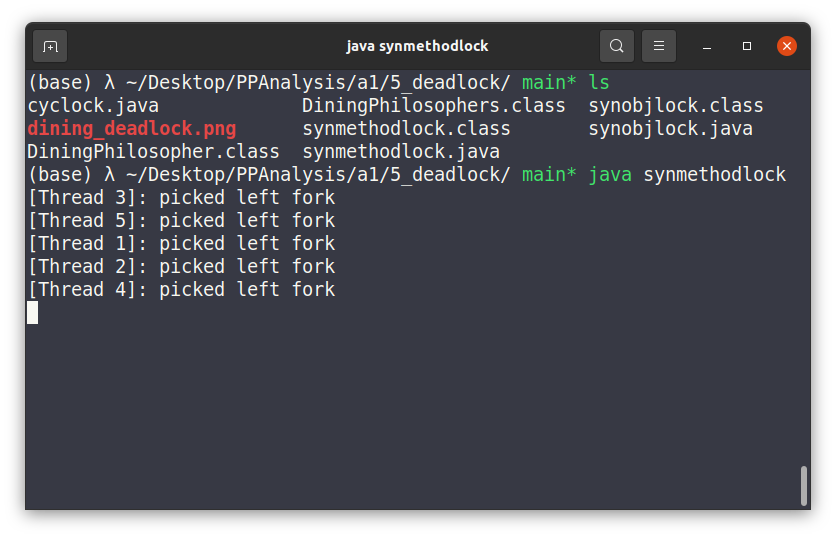
\includegraphics[scale=0.5]{5_deadlock/synchronized_method_deadlock.png}
        \caption{Output of code in \Cref{code::51}}
        \label{fig::51}
      \end{figure}

    \subsection{Using a CyclicBarrier}
      The code snippet in \Cref{code::52} spawns $N$ threads which print a message and then synchronize at a barrier. Once the barrier is tripped by the last thread, it is again reset (hence \textbf{cyclic}), and the last thread runs the barrier action.\\
      This barrier action involves spawning a new thread which again awaits at the same barrier(which is reset). Thus we have a cyclic dependency between the post-barrier thread, the cyclic barrier and the last thread, which are all waiting for each other. This leads to a deadlock between the last thread and the post-barrier thread.\\
      A screenshot of the execution is shown in \Cref{fig::52}
      
      \lstinputlisting[label={code::52},caption={Code implementing a cyclic barrier deadlock}]{5_deadlock/cyclicbarrierlock.java}

      \begin{figure}[ht]
        \centering
        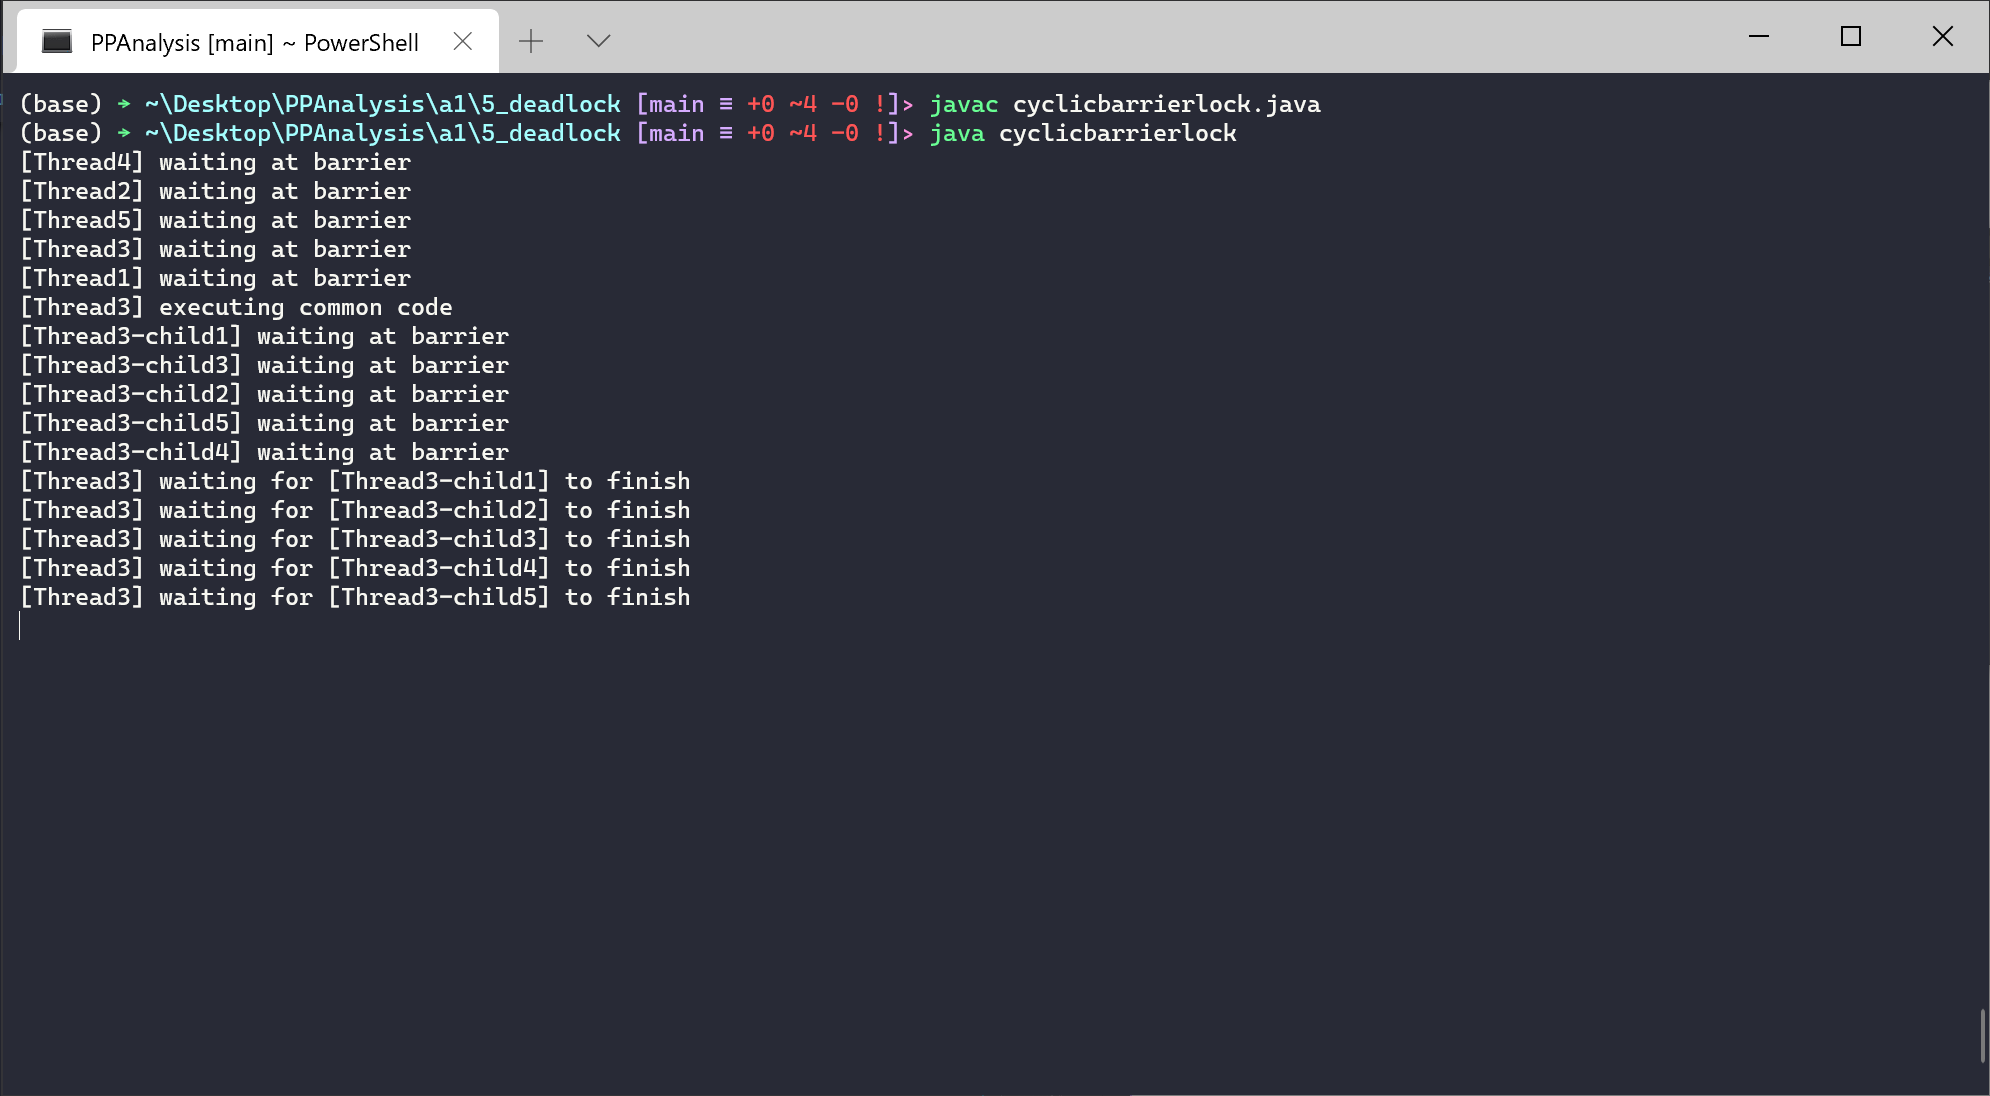
\includegraphics[scale=0.4]{5_deadlock/cyclic_barrier_deadlock.png}
        \caption{The cyclic barrier deadlock in action. }
        \label{fig::52}
      \end{figure}

\end{document}